\chapter{Object Selection}\label{cha:object_selection}

\section{Tracks and Vertices}\label{sec:object_selection:tracks_and_vertices}

\section{Electrons}\label{sec:object_selection:electrons}

Electrons can be identified with a high precision and large background rejection by matching clusters of energy
depositions in the electromagnetic calorimeter with extrapolations of reconstructed tracks provided by the ID\@.
To suppress background contributions from pile-up events or other objects like jets and hadronically decaying $\tau$-leptons
additional information of the ID and hadronic calorimeter are considered.

The identification algorithm~\cite{ATLAS-CONF-2016-024} is a likelihood-based method, which uses a multivariate analysis (MVA) technique to
evaluate multiple properties of the electron candidate.
Different requirements on the likelihood discriminant\footnote{The discriminant is defined as
$\frac{\mathcal{L}_S}{\mathcal{L}_S + \mathcal{L}_B}$, where $\mathcal{L}_S$ and $\mathcal{L}_B$ denote the product of
the signal and background probability density functions of the used variables.} yield different operating points,
labeled as  \emph{loose}, \emph{medium}, and \emph{tight}.
They provide a different level of electron identification efficiency and background rejection.

In this analysis the \emph{loose} criterion is chosen.
Additional requirements are $\pt > \unit[15]{GeV}$ and $\abs{\eta} < 2.47$.
The Pixel Detector and SCT can only provide information for reconstruction and identification in this $\eta$-range.
Electrons within $1.37 < \abs{\eta} < 1.52$ are excluded, because of the poor reconstruction and identification
performance caused by the crack between the barrel and end-calorimeters.

To increase the background rejection, isolation requirements are introduced by the following two discriminating variables.
The calorimetric isolation energy $\et^{\text{cone}0.2}$ is defined as the sum of transverse energy deposited within
$\dr = 0.2$ around the electron candidates.
Corrections for electron energy leakage, pile-up, and the underlying event activity are applied.
The sum of the transverse momentum of all tracks within $\dr = \min(0.2, \unit[10]{GeV} / \et)$ builds the
track isolation $\pt^{\text{varcone}0.2}$. The tracks need to fulfill certain quality requirements and have to originate
from the primary vertex.
Based on different selections criteria on quantities $\et^{\text{cone}0.2} / \et$ and
$\pt^{\text{varcone}0.2} / \et$ multiple operating points are constructed. This analysis uses the \emph{gradient}
isolation criterion with a targeted efficiency of
$\unit[0.1143]{\%} \times \et / \text{GeV} + \unit[92.14]{\%}$~\cite{ATLAS-CONF-2016-024}.

The efficiencies of the electron identification and isolation criteria are measured using a \emph{tag-and-probe technique}
in $\Z \to \epem$ and $\JPsi \to \epem$ events.
The \emph{tag} electron must pass the \emph{tight} identification criterion as well as some other selection criteria.
Because of the chosen events it is very probable that a second electron, the \emph{probe}, is contained in this event.
By counting how many \emph{probe} electrons pass the different identification and isolation requirements the efficiencies
of those working points can be obtained.
The combined reconstruction and identification efficiencies in $\Z \to \epem$ events as a function of $\et$ and $\eta$
are shown in \cref{fig:object_selection:el_id_eff}.
In account to correct for differences in data and simulated events the efficiencies are calculated for both event types.
The ratio is then used to derive \emph{scale factors}, which are applied to the simulated events in this analysis.

% TODO energy resolution

\begin{figure}[htb]
    \begin{center}
        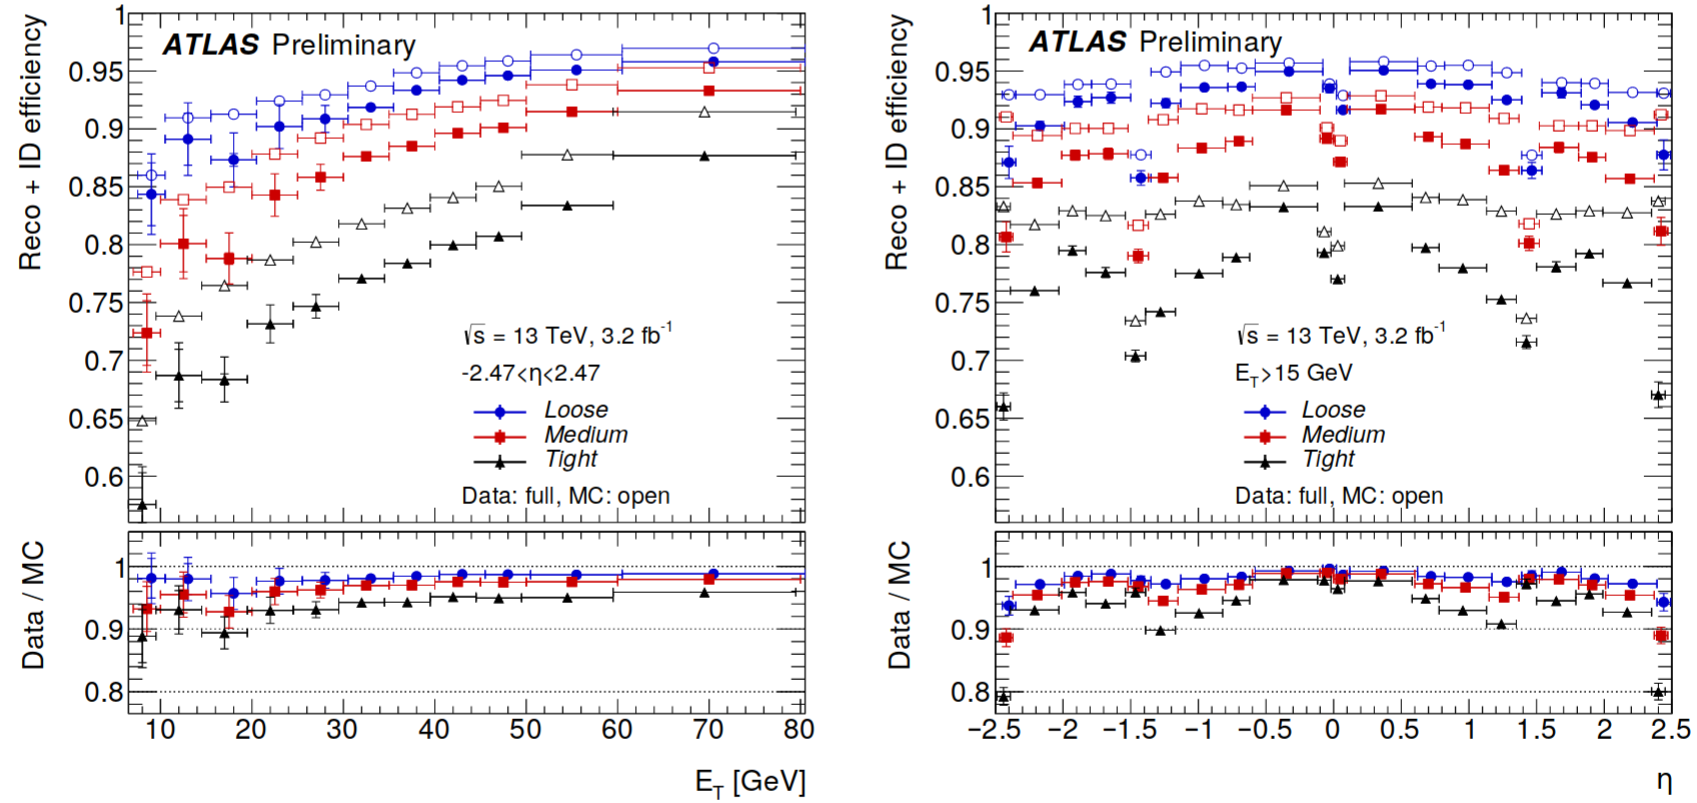
\includegraphics[width=0.9\linewidth]{./figures/object_selection/el_id_eff.png}
        \caption{Combined electron reconstruction and identification efficiencies for $\Z \to \epem$ events as a
                 function of $\et$ (left) and $\eta$ (right) for the \emph{loose}, \emph{medium}, and \emph{tight}
                 working points. The inner error bars show the statistical uncertainty, the outer error bars combine
                 the statistical and systematic uncertainties.~\cite{ATLAS-CONF-2016-024}}\label{fig:object_selection:el_id_eff}
    \end{center}
\end{figure}

\section{Muons}\label{sec:object_selection:muons}

\section{Jets}\label{sec:object_selection:jets}

\section{Tau Leptons}\label{sec:object_selection:tau_leptons}

\section{Missing Transverse Energy}\label{sec:object_selection:missing_transverse_energy}

\section{Overlap Removal}\label{sec:object_selection:overlap_removal}


